\section{Implementation Details}
\label{app:impl}

\begin{table}[!ht]
\caption{Fixed implementation and statistical settings.}
\label{tab:A2}
\centering
\small
\begin{tabular}{lp{0.68\linewidth}}
\toprule
\textbf{Component} & \textbf{Setting} \\
\midrule
Fault injection & Random scalar in prefill intermediate activations; two random bits flipped per execution; seed 42. \\
Projection & Per-layer 64D random projection with a consistent layer-index instrumentation seed 42 within a model. \\
Predictor & Layer-aware residual MLP: 16D source/target layer embeddings, hidden size 64, 8 residual blocks, dropout 0.1. \\
Predictor training & AdamW, learning rate 5e-4, weight decay 1e-4, batch size 2{,}048; at most 500 epochs; ReduceLROnPlateau and patience-10 early stopping. \\
Detector & XGBoost: learning rate 0.01, max depth 6, 10{,}000 trees, subsample/colsample 0.9, early stopping 500. \\
Threshold calibration and statistics & Maximize Significant-SDC F1 on the Validation set; nine-task macro average; per-task 95\% CI from image/question-group bootstrap with 10{,}000 resamples. \\
\bottomrule
\end{tabular}
\end{table}

\begin{figure}[!ht]
\centering
    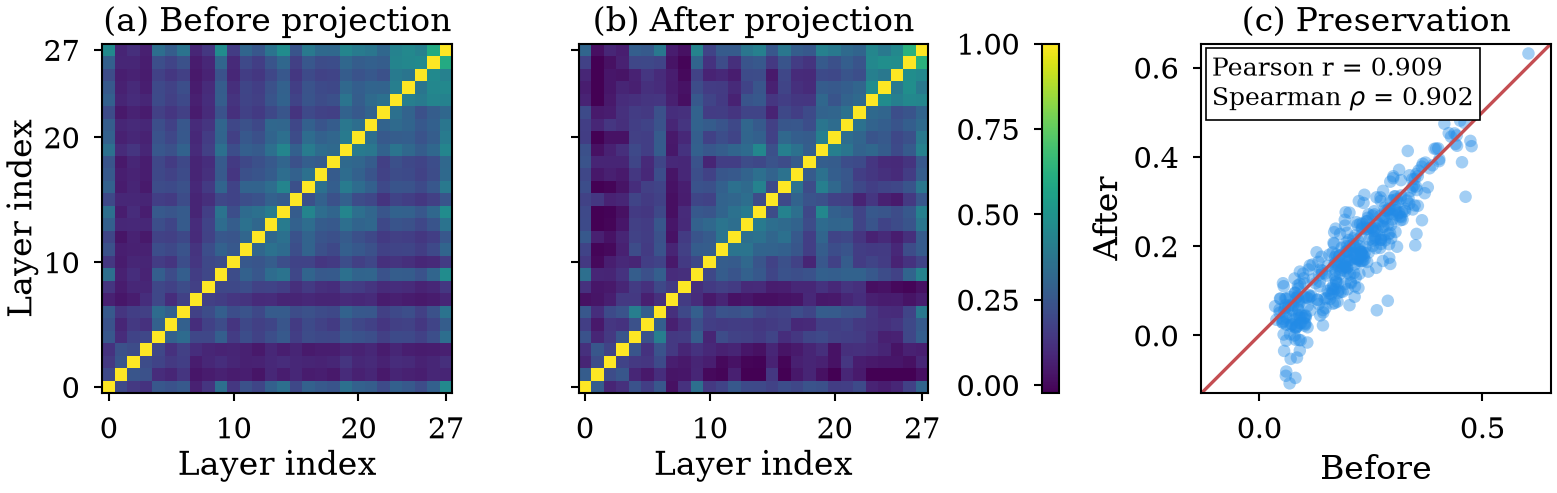
\includegraphics[width=0.9\linewidth]{Figures/figure5_projection_preservation.png}
    \caption{Feature structure preserved by the 64-dimensional column-orthogonal projection (Qwen2.5-VL-7B, LingoQA): pairwise similarity before vs. after projection.}
    \label{fig:jl}
\end{figure}

\begin{table}[!ht]
  \centering
  \caption{Nominal Inter-Layer Predictor performance on the group-disjoint 15\% predictor evaluation subset within the outer Training set.}
  \label{tab:fault_free_predictor_performance}
  \small
  \begin{tabular}{lcccccc}
    \toprule
    \multirow{2}{*}{Model}
      & \multicolumn{2}{c}{EarthVQA}
      & \multicolumn{2}{c}{LingoQA}
      & \multicolumn{2}{c}{VQAv2} \\
    \cmidrule(lr){2-3}
    \cmidrule(lr){4-5}
    \cmidrule(lr){6-7}
      & MSE & CosSim
      & MSE & CosSim
      & MSE & CosSim \\
    \midrule
    Qwen2.5-VL-7B
      & 0.0844 & 0.8589
      & 0.1451 & 0.7761
      & 0.2207 & 0.6934 \\
    InternVL3-8B
      & 0.0684 & 0.8117
      & 0.1094 & 0.7149
      & 0.1399 & 0.6367 \\
    LLaVA-1.5-7B
      & 0.0066 & 0.9138
      & 0.0162 & 0.7557
      & 0.0178 & 0.7326 \\
    \bottomrule
  \end{tabular}
\end{table}

